\documentclass[10pt]{article}

\usepackage{geometry}
\geometry{
	a4paper,
	total={6.85in, 9.92in},
	left=0.71in,
	top=0.63in,
}
\usepackage[utf8]{inputenc}
\usepackage{hyperref}
\usepackage{graphicx}
\usepackage{listings}

\pagenumbering{gobble}

\title{Porting the Excel 2000 ``Dev Hunter'' Easter Egg}

\makeatletter
\renewcommand{\maketitle}{
\begin{flushleft}
{\noindent\Huge\bf\@title}\break
\end{flushleft}
}
\makeatother

\begin{document}
\maketitle
\vspace{0.4em}

In \emph{Paged Out!} \#6 I described \textbf{Dev Hunter}, the hidden car-shooter
easter egg buried in Excel 2000's \texttt{MSOWC.DLL}, and a loader that runs it
outside Excel. You drive a highway hunting the Excel developers themselves, whose
names scroll past painted on the road as mock movie credits (``Stunts:
Additional'') between taunts like ``Pivot! Pivot! Pivot!'' and ``You will respect
the rectangles.'' But the loader still needs the original DLL, and Excel 2000
with its DirectDraw path only gets harder to run every year. I wanted to free the
game completely: reimplement it as a small standalone program --- no Excel, no
DirectDraw, no DLL --- that anyone can build, read, and play, so the easter egg
outlives its host. This time I didn't write it myself. I had an AI agent
(\textbf{Claude Code}, Anthropic's agentic coding tool) do the entire job ---
reverse-engineer \texttt{MSOWC.DLL} and translate the game into a standalone C++
program --- while I steered.

Working from Binary Ninja's decompilation, the AI rebuilt the
game from the recovered palette, decrypted developer text, RNG, and projection
constants, and translated the DLL's real \texttt{render} and rasterizer routines
into C. It built and ran, but the rendering was clearly off (Fig.~1, left):
developer names spilling off the tarmac, the road at the wrong scale, cars
reduced to blocks. The integer and pointer code came across faithfully; the
geometry, which runs entirely on the x87 FPU stack, is the kind of code
decompilers reconstruct imperfectly --- so the translation was subtly wrong, and
re-reading the listing wasn't fixing it.

\begin{figure}[h]
\centering
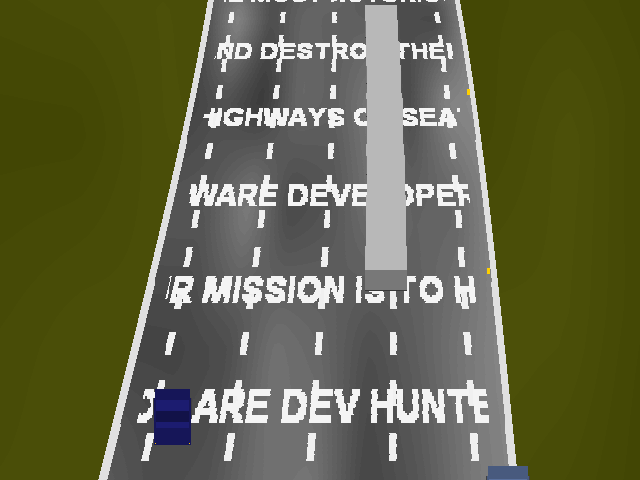
\includegraphics[width=0.49\linewidth]{before.png}\hfill
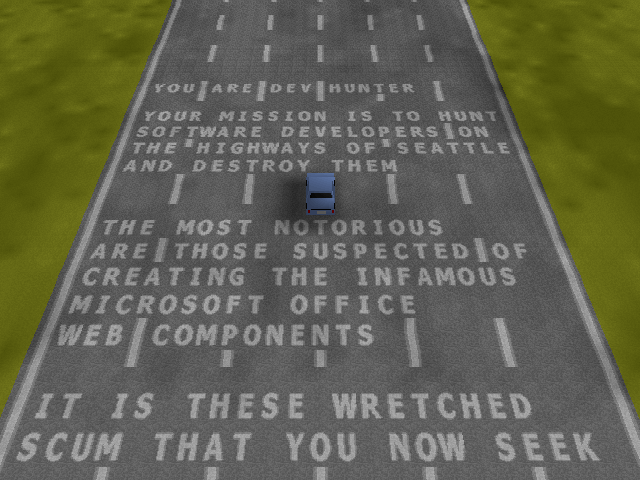
\includegraphics[width=0.49\linewidth]{after.png}
\caption{The same intro screen: the initial standalone build (left) vs.\ the
final debugger-verified port (right).}
\end{figure}

At this point I decided to intervene: I pointed the AI at the debugger, to
observe the program's real state instead of reading the code statically. The AI
turned that into an automated oracle --- it scripted Binary Ninja's headless debugger to
launch the game, break right before the DirectDraw \texttt{Unlock}, and read the
live 8-bit framebuffer at \texttt{*(this+0x34)} (pitch \texttt{*(this+0x20)}) plus
the entire $\sim$\texttt{0x9a96c}-byte game object, then diffed that ground truth
against its own port frame by frame and checked the physics by comparing the
object before and after a single \texttt{tick}. Each mismatch became an exact,
usually one-line fix (a sheared projection edge, a dropped floating-point value,
a bad texture mask).

The port is now \textbf{byte-identical} to the original across a
full day/night cycle. Getting a clean bit-for-bit comparison took two tricks: the
game's \texttt{init} --- terrain, textures, the 3-D letter atlas --- is
deterministic (RNG seed 0), so rather than re-derive its heavy x87 setup the port
loads a snapshot of \texttt{init}'s exact output and relocates its pointers; and
because the game times itself off the wall clock, headless runs only became
reproducible once a fixed virtual clock was wired in --- then SHA-256 over the
frame dumps could prove equivalence. The lesson: the AI could carry the whole
reverse-engineering port, but static decompilation only got it most of the way
--- the idea that closed the gap was a human one, giving it a debugger to observe
ground truth.

Source, build instructions, and a playable Win32 release:\\
\url{https://github.com/xusheng6/excel2000-devhunter-standalone}

\end{document}
